% ----------------------------------------------------------------
%% Thesis.tex -- MAIN FILE (the one that you compile with LaTeX)
%% ---------------------------------------------------------------- 



% Set up the document
\documentclass[a4paper, 11pt, oneside]{Thesis}  % Use the "Thesis" style, based on the ECS Thesis style by Steve Gunn
%\graphicspath{Figures/}  % Location of the graphics files (set up for graphics to be in PDF format)
\usepackage{fancyhdr}
% Include any extra LaTeX packages required
\usepackage[square, numbers, comma, sort&compress]{natbib}  % Use the "Natbib" style for the references in the Bibliography
\usepackage{verbatim}  % Needed for the "comment" environment to make LaTeX comments
\usepackage{vector}  % Allows "\bvec{}" and "\buvec{}" for "blackboard" style bold vectors in maths
\usepackage{graphicx} 
\usepackage{pdfpages}
\usepackage{float}  % Required for the [H] option in figures
\usepackage{acronym} % Required for the acronym environment
\usepackage[autostyle,german=quotes]{csquotes} % Required for the \enquote command
\usepackage{amsmath}  % Required for the \text command in maths mode
\hypersetup{urlcolor=blue, colorlinks=true}  % Colours hyperlinks in blue, but this can be distracting if there are many links.
%
%% ----------------------------------------------------------------
\renewcommand{\chaptername}{Kapitel}
\renewcommand{\tablename}{Tabelle}
\renewcommand{\bibname}{Literaturverzeichnis}
\renewcommand{\figurename}{Abbildung}
%% ----------------------------------------------------------------
\begin{document}
\begin{titlepage}

\newcommand{\HRule}{\rule{\linewidth}{0.5mm}} % Defines a new command for the horizontal lines, change thickness here

\center % Center everything on the page
 %----------------------------------------------------------------------------------------
%	LOGO SECTION
%----------------------------------------------------------------------------------------
\begin{minipage}{0.4\textwidth}
\begin{flushleft} \large

\includegraphics[width=5cm, height=1.2cm]{Pictures/UST.jpg}
\end{flushleft}
\end{minipage}

\begin{minipage}{0.4\textwidth}
\begin{flushright} \large

\includegraphics[width=5cm, height=1.2cm]{Pictures/ILH.jpg}
\end{flushright}
\end{minipage}\\[2cm]
 % Include a department/university logo - this will require the graphicx package
%----------------------------------------------------------------------------------------
%	HEADING SECTIONS
%----------------------------------------------------------------------------------------

\textsc{\LARGE \bfseries Fachpraktikum (Bachelor)}\\[0.2cm] % Name of your university/college
\textsc{\LARGE 6G Hardwarelabor - Design und Implementierung eines HF Transceivers}\\[0.2cm] 
%\textsc{\LARGE Design}\\[0.5cm] 
%\textsc{\Large ILH}\\[0.5cm] % Major heading such as course name
%\textsc{\large PuL-Analog Microwave Frontend Design}\\[0.5cm] % Minor heading such as course title

%----------------------------------------------------------------------------------------
%	TITLE SECTION
%----------------------------------------------------------------------------------------

\HRule \\[0.4cm]
{ \huge \bfseries Versuch 2: Auslegung eines HF-Verstärkers}\\[0.4cm] % Title of your document
\HRule \\[1.5cm]
 
%----------------------------------------------------------------------------------------
%	AUTHOR SECTION
%----------------------------------------------------------------------------------------
\textbf{Protokollführer}\\
{\large\ Lukas Müller}\\[0.2cm]
{\large\ Erik Zimmermann}\\[0.2cm]
{\large\ Farhad Valizada}\\[0.7cm]

\textbf{Betreuer}\\
{\large\ Simon Haussmann}\\[0.2cm]



%----------------------------------------------------------------------------------------
%	DATE SECTION
%----------------------------------------------------------------------------------------
\textbf{Eingereicht}\\
{\large \today} % Hier bitte am Tag der Abgabe das Datum eintragen
\\[0.2cm]

 
%----------------------------------------------------------------------------------------

\vfill % Fill the rest of the page with whitespace

\end{titlepage}

\clearpage

\pagenumbering{arabic}
\pagestyle{fancy}
\fancyhf{}
\fancyfoot[C]{\thepage} % Seitenzahl unten zentriert
\renewcommand{\headrulewidth}{0pt}

% Ensure every chapter resets the pagestyle to fancy
\let\oldchapter\chapter
\renewcommand{\chapter}{\clearpage\pagestyle{fancy}\oldchapter}

%% ----------------------------------------------------------------

% The Abstract Page


%% ----------------------------------------------------------------

\setstretch{1.3}  % Reset the line-spacing to 1.3 for body text (if it has changed)

% The Acknowledgements page, for thanking everyone
%\acknowledgements{
%\addtocontents{toc}{\vspace{1em}}  % Add a gap in the Contents, for aesthetics
%
%The acknowledgements and the people to thank go here, don't forget to include your project advisor\ldots
%
%}
%\clearpage  % End of the Acknowledgements1
%% ----------------------------------------------------------------

%\pagestyle{fancy}  %The page style headers have been "empty" all this time, now use the "fancy" headers as defined before to bring them back




\renewcommand{\contentsname}{Inhaltsverzeichnis}
\tableofcontents
\newpage

\chapter*{Abkürzungsverzeichnis}
\addcontentsline{toc}{chapter}{Abkürzungsverzeichnis}
\begin{acronym}[XXXXXX] % Adjust the width of the longest acronym
    \acro{ADS}{Advanced Design System}
    \acro{HF}{Hochfrequenz}
    \acro{6G}{Sixth Generation}
    \acro{SMA}{SubMiniature version A}
    \acro{PCB}{Printed Circuit Board}
\end{acronym}

\chapter{Einleitung(Farhad)}
\section{Relevanz der Funkübertragung im Alltag}
Jeden Tag nutzen wir Funkübertragungen in verschiedenen Formen, sei es durch WLAN, Bluetooth oder Mobilfunk. Diese Technologien ermöglichen es uns, Daten über große Entfernungen zu übertragen, ohne physische Verbindungen herstellen zu müssen. Die Grundlagen der Modulation sind entscheidend für die Entwicklung und Verbesserung dieser Technologien.
Die \ac{6G} der Funkübertragung ist die neueste Generation der Funkkommunikation, die eine höhere Datenrate, geringere Latenz und verbesserte Zuverlässigkeit verspricht. Sie ist aktuell in der Entwicklung, 
jedoch besteht bei dem Frequenzbereich von \ac{6G}, beginnend mit Sub-6 GHz (unter 6 GHz) bis hin zu THz-Bereich (100 GHz - 1 THz), 
die Herausforderung, dass die Signale bei höheren Frequenzen stärker gedämpft werden und somit eine höhere Signalstärke erforderlich ist, um eine zuverlässige Kommunikation zu gewährleisten.
Deswegen ist es leichter, eine beispielhafte Funkübertragung bei kleineren Abständen zu dimensionieren, um das Wissen bei größeren Strecken anwenden zu können.
\section{Ziel des Versuchs}
Das Ziel des heutigen und des letzten Versuchs ist es, eine Bildübertragung über eine Funkverbindung zu realisieren und dabei die Grundlagen der Bildübertragung mithilfe von 6G zu verstehen.
Dies bietet einen guten Einblick in die digitale Kommunikation und die Modulation von Signalen, die für die Übertragung von Daten über Funkverbindungen unerlässlich ist.
\clearpage 

\chapter{Theoretische Grundlagen(Lukass)}
\section{Modulationsarten}

\section{Blockdiagramm einer Sendestrecke}
\subsection{DAC}
\subsection{LO}
\subsection{Mischer} 
\subsection{PA}
\subsection{Antennen}
\subsection{LNA}
\subsection{Demodulation}
\subsection{ADC}
\section{Mathematische Grundlagen: Fourier-Transformation}
\subsection{Betrag und zeitlicher Verlauf von Rechteckfunktion}
\subsection{Betrag und zeitlicher Verlauf von Sinusfunktion}
\subsection{Multiplikation der beiden Funktionen im Zeitbereich}
\section{Zusammenhang von Datenrate und Bandbreite}
blabla
\clearpage
\label{chapter:theoretische_grundlagen}

\chapter{Hochfrequenz-Simulation(Charhad)}

\section{Inbetriebnahme von Keysight Advanced Design System (ADS)}
\subsection{Installation von ADS}
Die Software \ac{ADS} dient zur Simulation von Schaltungen verschiedener Komplexitätsgrade. 
In diesem Versuch wird die Software verwendet, um eine Hochfrequenzschaltung zu simulieren und zu analysieren. 
Die Software bietet eine Vielzahl von Funktionen, darunter die Möglichkeit, Schaltungen zu entwerfen, S-Parameter zu simulieren und verschiedene Analysewerkzeuge zu verwenden.
\section{DC-Simulation}
\subsection{Erstellen eines neuen Projekts}
Die Software ist auf den Rechnern im Labor bereits installiert gewesen. 
Nach dem Start der Software wird ein neues Projekt aus den bereits zur Verfügung stehenden Workspaces erstellt. 
Diese sind auf der ILIAS-Seite des Praktikums in dem Dateiarchiv \texttt{TransmitterAmpDesign 2024.zip} hinterlegt. 
Die Datei wird entpackt und in der Software geöffnet. Außerdem werden die benötigten Bibliotheken aus dem Dateiarchiv \texttt{Infineon-RFTransistor-Keysight ADS Design Kit-SM-v02 10-EN.zip} geladen, diese stehen ebenfalls auf der ILIAS-Seite zur Verfügung.
\section{Analyse des Datenblattes zu Transistor BFR181W}
Die maximal zulässige Kollektorstrom $I_{C,\mathrm{max}}$ beträgt 20\,mA.
\section{S-Parameter Simulation}

blabla
\clearpage

\label{chapter:hf_simulation}

\chapter{Technische Umsetzung(Erik)}
\section{Platinenaufbau}
Die Platine ist mit mehreren Bauteilen ausgestattet, die bis auf drei selbst zu dimensionierende Widerstände bereits vollständig bestückt ist.

Zur Erklärung von Abbildung 4.1 hier eine kurze Information zu den wichtigsten Abkürzungen:
\begin{itemize}
    \item R: Widerstand
    \item C: Kondensator
    \item J: Stecker/Relais
\end{itemize}

Die wichtigsten Bauteile sind:
\begin{itemize}
    \item J1: Anschluss an den FieldFox (Ausgangssignal)
    \item J40: Verbindung zum Oszillator (Taktquelle für die Schaltung) und Anschluss an den FieldFox (Eingangssignal)
    \item R47-49: Widerstände zur Arbeitspunkteinstellung
    \item Oszillator (XLL536C50.000000X): HF-Taktsignal
    \item Transistor (BFR181W)
    \item Operationsverstärker (U20-LMV651MG/NOPB; U21-NCX2200GW,125)
    \item USB-UART-IC (FT232RL)
\end{itemize}

\begin{figure}[h]
    \centering
    \includegraphics[width=1.0\textwidth]{Pictures/Bestückungsplan.jpg}
    \caption{Bestückungsplan}
\end{figure}

\section{Bestückung der PCB}
Die in Kapitel 3 bestimmten Widerstände werden nun im Rahmen der praktischen Umsetzung der Schaltung auf die bereits vorbereitete Platine angebracht. Auf dem Bestückungsplan entspricht R47 dem Widerstand R3 mit 1000~Ohm, R48 dem Widerstand R4 mit 4700~Ohm und R49 dem Widerstand R5 mit 330~Ohm. Beim Löten der drei Widerstände wird auf eine saubere und präzise Löttechnik geachtet, um die gewünschte elektrische, mechanische und HF-technische Funktion der Schaltung zu garantieren.
\begin{figure}[h]
    \centering
    \includegraphics[width=0.54\textwidth]{Pictures/Platinebestückt.jpg}
    \caption{Bestückte Platine}
\end{figure}

\section{DC-Pegel verifizieren}
Nach dem Bestücken der Platine wird die Funktionalität der Schaltung überprüft. Hierzu wird eine Versorgungsspannung von 4,8~V angelegt, um die Gleichspannungspegel an den relevanten Punkten der Schaltung zu überprüfen. Die abfallenden Spannungen werden mit einem Oszilloskop gemessen. Relevant sind die Spannungsabfälle über R47, R48 und R49. Diese gemessenen Spannungen werden mit den idealen Werten der Simulation verglichen.
\clearpage
\section{SOLT-Kalibrierung}
Das Ziel der SOLT-Kalibrierung (Short, Open, Load, Through) ist die Eliminierung von systematischen Messfehlern, die durch die Messeinrichtung (Kabel, Adapter etc.) selbst entstehen und die Messung verfälschen.
Durch das Messen dieser Fehler lässt sich die Messung korrigieren.
Dafür werden vier verschiedene Kalibrierstandards benötigt:
\begin{itemize}
    \item Short (Kurzschluss): Ein Kurzschluss-Standard wird an den Messport des VNAs angeschlossen. Da ein idealer Kurzschluss alle Leistung reflektiert und eine Phasenverschiebung von 180 Grad verursacht, misst der VNA diese Referenz. Abweichungen vom Ideal werden erfasst.
    \item Open (Leerlauf): Ein Leerlauf-Standard wird angeschlossen. Ein idealer Leerlauf reflektiert ebenfalls die gesamte Leistung, jedoch mit einer Phasenverschiebung von 0 Grad. Auch hier werden Abweichungen aufgezeichnet.
    \item Load (Abschluss/Last): Ein Präzisions-Abschlusswiderstand (meist 50~Ohm) wird angeschlossen. Ein idealer Abschlusswiderstand absorbiert die gesamte Leistung ohne Reflexion. Dies dient dazu, die Leistungsanpassung des Systems zu kalibrieren.
    \item Through (Durchgang): Bei einer 2-Port-Messung wird ein direkter Durchgang (ein kurzes, bekanntes Kabel oder ein Adapter) zwischen den beiden Messports des VNAs angeschlossen. Dies ermöglicht die Kalibrierung der Übertragungseigenschaften zwischen den Ports und die Korrektur von Phasen- und Amplitudenfehlern des Übertragungspfades.
\end{itemize}
\begin{figure}[h]
    \centering
    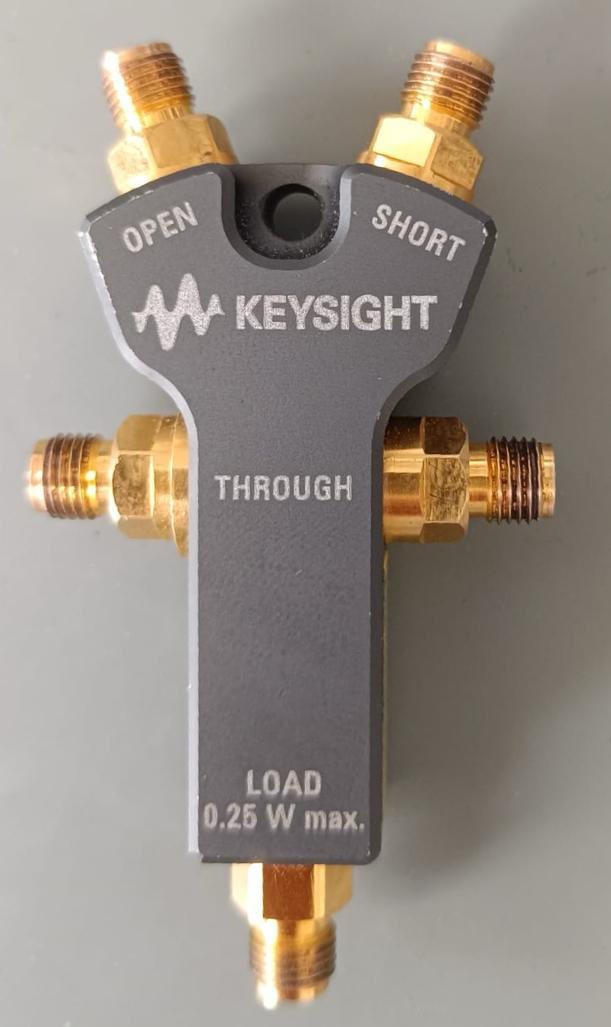
\includegraphics[width=0.25\textwidth]{Pictures/Keysightkallibrierung.jpg}
    \caption{Kalibrierung am Keysight FieldFox}
\end{figure}
\clearpage

Die Kalibrierung wird am Keysight FieldFox durchgeführt. Sie erfolgt über sieben Schritte, die vom Gerät angeleitet werden. Danach ist das Gerät bereit für die Messung.
\subsection{Verfizierung der Qualität der SOLT-Kalibrierung}
Unter Beibehaltung des Messaufbaus werden nun die S-Parameter, der bei der Kalibrierung verwendeten Kabel, betrachtet. Ist die Kalibrierung gelungen sollte unter optimalen Bedingungen bei den Streuparametern keine Dämpfung mehr angezeigt werden, da die Kalibrierung die Kabeldämpfung herausrechnet. In unserem Fall ist die zeigt die Messung eine kleine Abweichung, ist jedoch sehr nahe am Optimum. Es ist daher keine erneute Kalibrierung von Nöten.


\section{Vergleich zur Simulation}
Die Simulation wurde, wie zuvor beschrieben, mit der Software Advanced Design System (ADS) durchgeführt. In der Simulation fällt über R47 eine Spannung von 0,811~V, über R48 eine Spannung von 3,989~V und über R49 eine Spannung von 1,27~V ab. Wir überprüfen nun, ob sich unsere Messung mit den simulierten Werten deckt.

\begin{table}[h]
    \centering
    \begin{tabular}{|l|l|l|}
        \hline
        \textbf{Widerstand} & \textbf{Simulation [V]} & \textbf{Messung [V]} \\
        \hline
        R47 & 0{,}811 & 0{,}809 \\
        \hline
        R48 & 3{,}989 & 3{,}991 \\
        \hline
        R49 & 1{,}27  & 1{,}26 \\
        \hline
    \end{tabular}
    \caption{Vergleich von simulierten und gemessenen Spannungswerten}
\end{table}

\clearpage


\chapter{Diskussion der Ergebnisse(GangBang)} %Diskussion über die Qualität der Ergebnisse
\section{Vergleich von Theorie und Praxis}
\section{Erklärung von Abweichungen}
bla bla
\clearpage
\label{chapter:diskussion}

\chapter{Fazit(Jeder)}

Im Verlauf dieses Versuches konnten wir die grundlegende Funktionsweise eines Coupled Line Filters praktisch nachvollziehen und ebenfalls unser theoretisches Wissen erweitern. Es ist sehr interessant zu sehen, wie sich die anfangs unscheinbaren Platine zu einem komplexen Konstrukt entwickelt deren einzelnen Komponenten und deren Zusammenspiel wir nach und nach immer besser verstehen. Ebenfalls ist die Arbeit mit der Simmulationssofware ADS äußerst erkenntnisreich und hilft uns die Fehler in dem praktischen Teil des Versuches zu identifizieren und zu sehen, wie es unter optimalen Bedingungen aussehen müsste. Es gibt noch vieles zu lernen im Verlauf dieses Praktikums und wir sind gespannt auf das was noch kommt. 
\clearpage  
\label{chapter:fazit}

\renewcommand{\bibname}{Literaturverzeichnis}
\addcontentsline{toc}{chapter}{Literaturverzeichnis}
\input{Chapter/literaturverzeichnis}

\end{document}  % The End
%% ----------------------------------------------------------------
